\section{Additional Complete Loss Trajectories}
\label{app:supporting-loss}
\begin{figure}[t]
\centering
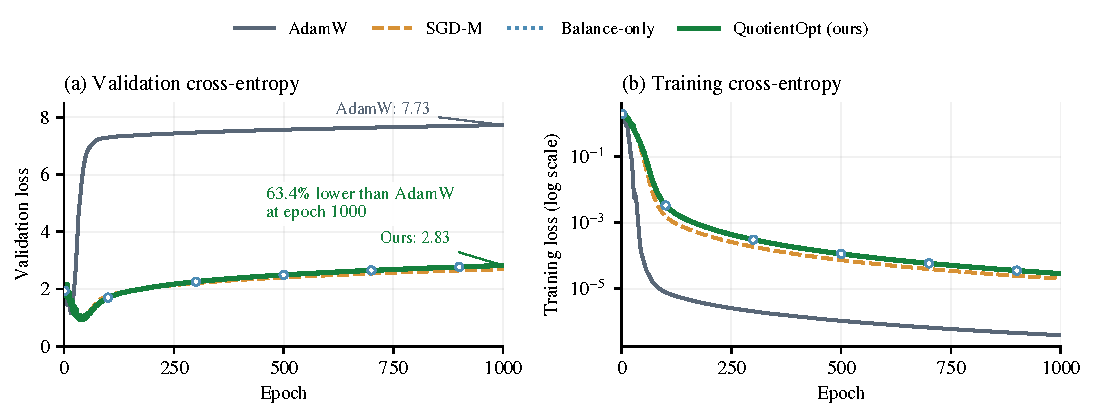
\includegraphics[width=.99\linewidth]{figures/core_loss_cora.pdf}
\caption{\textbf{Core loss curves: lower validation loss than AdamW.}
Cora/GCN input adapter, rank 4, seed 42, $\beta=0.9$.
The complete seven-learning-rate block selects $\eta=10^{-2}$ for
every method using validation accuracy; test metrics do not enter
selection. All 1000 raw epoch observations are shown without smoothing
or interval truncation. (a) Validation cross-entropy: QuotientOpt's
final loss is $63.4\%$ below AdamW's, while SGD-M is slightly lower
and balance-only nearly overlaps QuotientOpt. Open green circles
identify the overlapping balance-only trajectory.
(b) Training cross-entropy on a logarithmic scale: AdamW attains
the smallest training loss.}
\label{fig:core-loss}
\end{figure}
\begin{figure}[t]
\centering
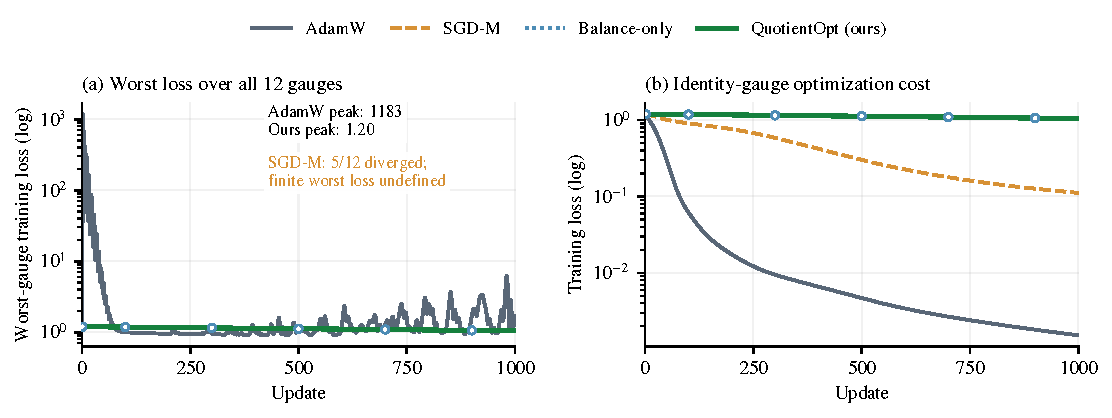
\includegraphics[width=.99\linewidth]{figures/core_loss_gauge.pdf}
\caption{\textbf{Core sensing loss curves: robustness and optimization cost.}
True rank-one sensing, $128\times128$, rank 16, 19,200 observations,
seed 42, $\eta=10^{-3}$, $\beta=0.9$; all 1000 raw observations
and logarithmic loss axes. (a) At each update, the maximum training
loss over every one of the 12 prescribed gauges. AdamW and both
balanced arms have all 12 completed trajectories. The five confirmed
SGD-M failures preclude a finite 12-gauge envelope; an envelope of
only its successful cases is not substituted.
(b) The identity-gauge reference: AdamW fits this problem much better
at the fixed learning rate. Both panels retain the overlapping
balance-only control. The gain in (a) is gauge robustness, not faster
identity-gauge recovery or an accuracy gain uniquely due to projection.}
\label{fig:core-gauge-loss}
\end{figure}
\begin{figure}[t]
\centering
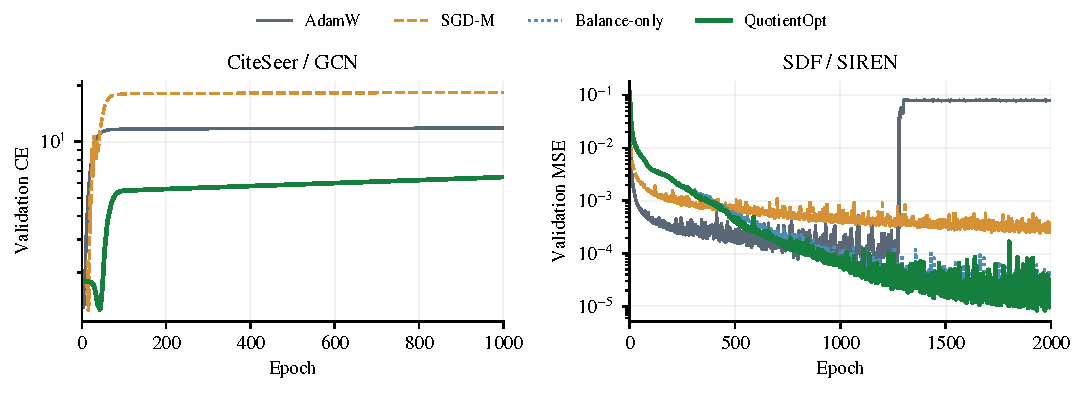
\includegraphics[width=.99\linewidth]{figures/new_task_validation_cases.pdf}
\caption{Exploratory validation-loss case studies from completed new-task blocks. The presentation rule requires at least 1\% lower minimum validation loss for a full-horizon QuotientOpt run than AdamW, including its best finite stopped-trial checkpoints; test outcomes do not select panels. Every method receives the same thirteen-setting optimizer budget and every selected trajectory is shown in full. All four methods are retained. This selected-case figure does not establish improvement over every baseline. All tasks, test metrics, and unfavorable outcomes are retained in Table~\ref{tab:new-task-scores} and Appendix~\ref{app:new-task-expansion}.}
\label{fig:new-task-validation-cases}
\end{figure}
\begin{figure}[t]
\centering
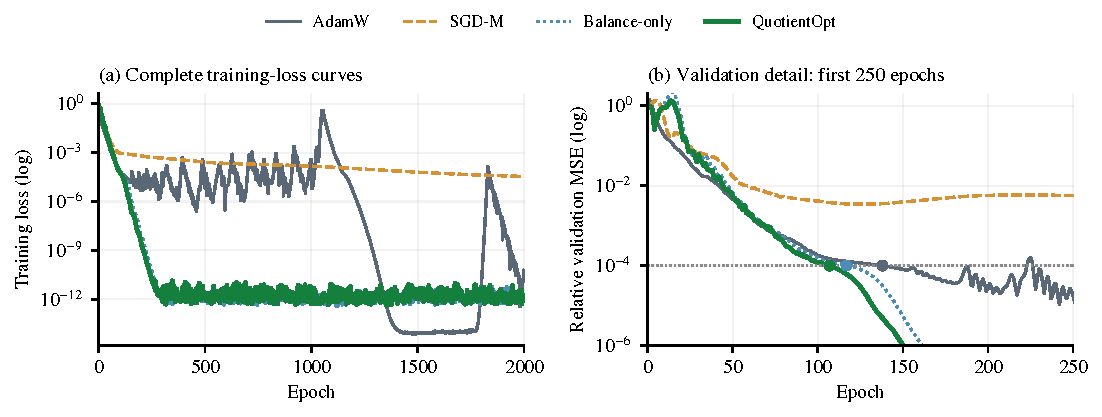
\includegraphics[width=.99\linewidth]{figures/new_matrix_convergence_raw.pdf}
\caption{\textbf{Additional matrix-completion loss curves.} Rank 8, planted condition 100, $128\times128$, seed 42. Each method selects its setting by the earliest validation epoch reaching $10^{-4}$ of the common initial validation MSE, over the same 13-setting budget. For SGD-M, which never reaches the target, the minimum-validation-loss full-horizon setting is shown. (a) Complete raw training-loss observations, without smoothing. (b) A common first-250-epoch validation zoom, with first-hitting points and the target line. These are actual selected-run trajectories. Figure~\ref{fig:new-task-convergence} separately reports tuning envelopes; the full record includes every setting and stopped prefix.}
\label{fig:new-matrix-raw}
\end{figure}
\begin{figure}[t]
\centering
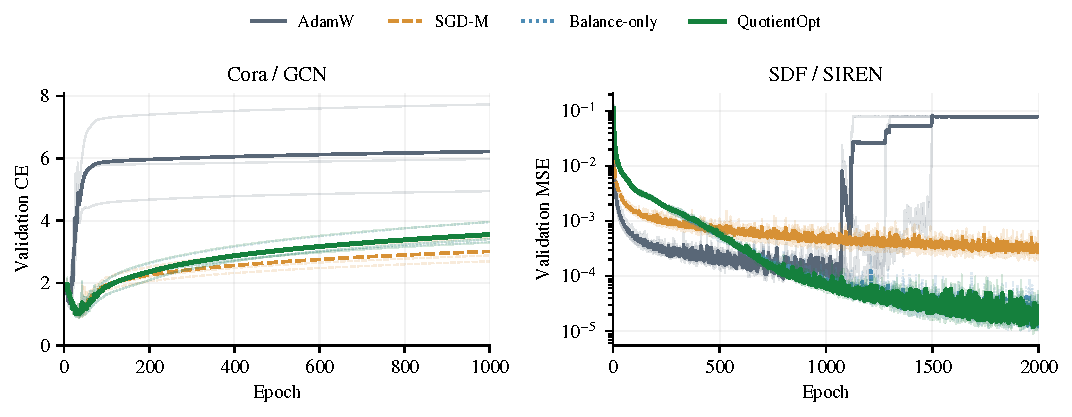
\includegraphics[width=.99\linewidth]{figures/initialization_confirmation_curves.pdf}
\caption{\textbf{Conditional initialization loss checks.} Data and shuffle seed 42 are fixed, with model initializations 42, 43, and 44. Parent-selected learning rates are frozen per method, with no per-initialization retuning. Thin lines show every initialization; thick lines show their arithmetic mean validation loss at each epoch. All raw epochs are retained without smoothing. The mean curves are descriptive summaries, not confidence bands. Test outcomes and all four controls are retained in Table~\ref{tab:initialization-confirmation}.}
\label{fig:initialization-loss}
\end{figure}
\FloatBarrier
